\chapter{More on effective constitutive modeling of soft tissues, kinematics, parameter correlation, and form.}

\section*{Preface}
\addcontentsline{toc}{section}{Preface}%

In this appendix, we cover some of the lose ends for the effective constitutive models (chapter 5) we developed and as well as some of the considerations and tests we have done that were not included in the main text. First we will look at the choice of kinematic variable and how they affect the constitutive model. They we will look at how this choice will affect the parameter correlations, stress and elasticity tensor forms, and thus how we arrived at the choice of Green-Lagrange strain for our effective constitutive model. We will also go into more detail about the optimal loading paths, how they develop as you are additional loading paths. Finally, we will go into a deeper look at the effect of changing the effective model form and loading paths of the ability of the model to fit and predict mechanical responses. 



%---    INTRODUCTION
%%%%%%%%%%%%%%%%%%%%%%%%%%%%%%%%%%%%%%%%%%%%%%%%%%%%%%%%%%%%%
%%	Constitutive model form									%
%%%%%%%%%%%%%%%%%%%%%%%%%%%%%%%%%%%%%%%%%%%%%%%%%%%%%%%%%%%%%

\section{Effective constitutive model formulation}\label{sec:greenvshencky}

%-----------------------------------------------------------
%	Kinematics
%-----------------------------------------------------------
% \subsection{Kinematic considerations}


% 	The invariants and pseudo-invariants of the right or left Cauchy Green tensor is the most popular for constitutive models of soft tissues. Indeed, we use them often with our structural models \cite{fata_insights_2014, zhang_meso_2016, Avazmohammadi2017b, sacks_novel_2016, zhang_modeling_2017}. There is a large number of invariants, each describes a facet of deformation: isotropic, volumetric strain, anisotropic, or interactions between them. The breadth of choices, allows for more freedom in selecting a combination for constitutive models that best describes the mechanisms in the tissue. Each invariant describes a facet of deformation: isotropic, volumetric strain, anisotropic, or interactions between them. The three isotropic invariants of the right Cauchy Green tensor are $I_1 = Tr(\mathbf{C})$, $I_2 = \frac{1}{2}\left( Tr(\mathbf{C})^2 - Tr(\mathbf{C}^2)\right)$, $I_3 = \det(\mathbf{C})$. The extension for anisotropic materials is summarized by Holzapfel \cite{holzapfel_nonlinear_2000}. The usual starting point is $I_4 = \mathbf{m}\cdot \mathbf{C} \mathbf{m}$, where $\mathbf{m}$ is a unit vector for material axis, or the preferred direction, most commonly that of the constituent fibers, such as collagen and elastin. Other pseudo invariants include $I_5 = \mathbf{m}\cdot \mathbf{C}^2 \mathbf{m}$, $I_6$ and $I_7$ which are equivalent of $I_4$ and $I_5$ for another family of fibers along some $\mathbf{n}$, $I_8 = \mathbf{m}\cdot\mathbf{C}\mathbf{n}$ and $I_9 = (\mathbf{m}\cdot\mathbf{n})^2$ can be used to describe the interaction between these two fiber families \cite{sacks_novel_2016}\cite{avazmohammadi_novel_2017}, etc. 
	
	
% 	In a generalized model, where no assumptions can be made on the behaviors and mechanisms of the tissue,  the use of invariants do not lend itself to creating a single generalized form. One example is when modeling the effects of fiber rotation in tissues with widely distributed fiber orientations. This is one of the most difficult behavior to model using phenomenological approaches. Fiber rotation manifests as coupling interactions between axial stretches in the mechanical response of soft tissues. Invariant based models cannot easily reproduce this effect. One approach is to use the Driessen model \cite{driessen_structural_2005}, where additional fiber families are added until it can match the response of the soft tissue. However, this significantly increases computational costs and requires two additional parameters for each additional fiber family. Further extensions to this approach is to incorporate the fiber orientation distribution directly, such as in meso-scale structural approaches \cite{sacks_incorporation_2003a, fata_insights_2014, zhang_meso_2016}. However, this also increases the complexity and computational cost of the model, which defeats the point of phenomenological approaches entirely. Adding coupling invariants such as $I_8$ and $I_9$ are also an option. However, the inherent similarities between these invariants makes it a difficult choice to incorporate in a generalized constitutive model form. 

    
%     For the most part, it is easy to convert strains to other types. Even 
    
    
% 	The components of strain tensors, such as the Green-Lagrange, $\mathbf{E}$, right Cauchy-Green, $\mathbf{C}$, left Cauchy-Green, $\mathbf{B}$, or the right stretch, $\mathbf{U}$ can be used directly in the constitutive model. Although it is easy to convert them to each other, One example using strain tensor components is the commonly used generalized Fung model \cite{fung_biomechanics_1993}. The effects of choice of strain tensor is not entirely clear. Specifically, $\mathbf{U}$ scales linear with the deformation, whereas $\mathbf{E}$, $\mathbf{C}$, and $\mathbf{B}$ scales quadratically with the deformation. Functionally, these tensors behave very similarly. For example, $\mathbf{E}$ is just $\mathbf{C}$ scaled by $1/2$. More often than not, the choice is to simply default to $\mathbf{E}$, which leads to a simple mathematical form for the stress-strain relationship and the elasticity tensor. 

%-------	Hencky strains		-------%

    One additional strain basis we have considered is the Hencky strains, which is the logarithmic strain calculated from the upper triangular decomposition of the deformation gradient tensor with respect to the material axis as described in Criscione \textit{et al.} \cite{criscione_experimentally_2003a} and then further expanded on by Srinivasa \cite{srinivasa_use_2012} and Freed \cite{freed_logarithmic_2015, freed_conjugate_2017, erel_stress/strain_2017}. This has the following number of advantages: (1) The decomposed strains are easy to interpret physically, (2) it results in an extremely simple mathematical form the Cauchy stress, (3) the logarithmic strains are beneficial when dealing with experimental errors in reference configurations, and (4) It is expected to be slightly less correlated in comparison to the Green Lagrange strains. The Hencky strains have the greatest in difference compared to the Green-Lagrange strains, and are thus a good choice for comparing the strain bases.
    
    
%%%%%%%%%%%%%%%%%%%%%%%%%%%%%%%%%%%%%%%%%%%%%%%%%%%%%%%%%%%%
%-------------------	begin FIGURE 	-------------------%
\begin{figure}
\centering
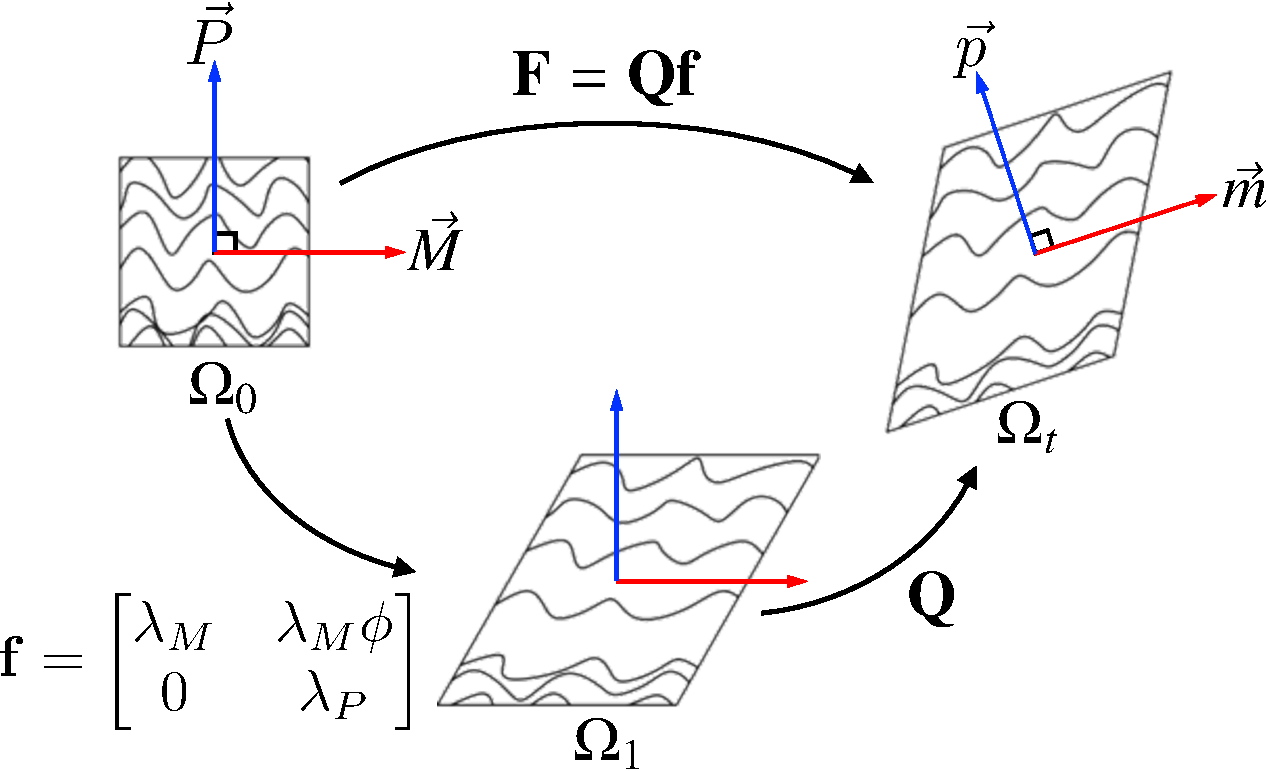
\includegraphics[width=5in]{Images/chapter5/henckykinematics}
\caption{The upper triangular decomposition of the deformation gradient tensor with respect the preferred material axis of soft tissues, whose components are used to define the Hencky strains.}
\label{fig:henckykinematics}
\end{figure}
%-------------------	 end FIGURE 	-------------------%
%%%%%%%%%%%%%%%%%%%%%%%%%%%%%%%%%%%%%%%%%%%%%%%%%%%%%%%%%%%%
    
    
    The Hencky strains can be formulated as followed. Briefly, the upper triangular decomposition, $\mathbf{f}$, when expressed with respect to the material axis of the tissue is given by
%==========================================================%
%-------------------	begin EQUATION 	-------------------%
\begin{equation}
\begin{aligned}
\left[\mathbf{f}\right]_{\mathbf{m}_0,\mathbf{n}_0} = \begin{bmatrix}
\lambda_m 	& \lambda_m\phi \\
0			& \lambda_n
\end{bmatrix}.
\end{aligned}\label{eqn:uppertriangulardecomposition}
\end{equation}
%-------------------	 end EQUATION 	-------------------%
%==========================================================%
    Here, $\mathbf{m}_0$ is the material axis in the referential configuration, which is generally the preferred direction of the fibers embedded in the tissue, $\mathbf{n}_0$ is the direction perpendicular to $\mathbf{m}_0$, $\mathbf{m}_t$ is the material axis in the deformed configuration, $\mathbf{n}_t$ is the direction perpendicular to $\mathbf{m}_t$, $\lambda_m$ and $\lambda_n$ are the stretches along these axes respectively, and $\phi$ is the angle of shear between $\mathbf{m}_0$ and $\mathbf{n}_0$. The corresponding deformation gradient tensor can thus be expressed as 
%==========================================================%
%-------------------	begin EQUATION 	-------------------%
\begin{equation}
\begin{aligned}
\mathbf{F} = \lambda_m\mathbf{m}_t\otimes\mathbf{m}_0 + \lambda_m\phi\mathbf{m}_t\otimes\mathbf{n}_0 + \lambda_n\mathbf{n}_t\otimes\mathbf{n}_0.
\end{aligned}
\end{equation}
%-------------------	 end EQUATION 	-------------------%
%==========================================================%
    The Hencky strains ($\gamma_1, \gamma_2, \gamma_3$), which are functions of the components of $\mathbf{f}$, can be determined using, 
%==========================================================%
%-------------------	begin EQUATION 	-------------------%
\begin{subequations}\label{eqn:henckystrains}
\begin{align}
\gamma_1 &= \log(\lambda_m), &	\gamma_2 &= \log(\lambda_n), 	& \gamma_3 &= \phi	\\
\lambda_m &= \mathbf{m}_t\cdot\mathbf{F}\mathbf{m}_0, &	\lambda_n &= \mathbf{n}_t\cdot\mathbf{F}\mathbf{n}_0,	&	\phi &= \left(\mathbf{m}_t\cdot\mathbf{F}\mathbf{m}_0\right)^{-1}\mathbf{m}_t\cdot\mathbf{F}\mathbf{n}_0.
\end{align}
\end{subequations}
%-------------------	 end EQUATION 	-------------------%
%==========================================================%
    
    
%-------	Hencky vs. Green-Lagrange strain	-------%

	We are most interested in the difference between Green-Lagrange and the Hencky strains for the formulation of the effective constitutive model (Summary Table \ref{tb:greenvshencky}). Firstly, as stated above , Hencky strains lead to a very convenient form for the Cauchy stresses,
%==========================================================%
%-------------------	begin EQUATION 	-------------------%
\begin{equation}\label{eqn:cauchystressform}
\mathbf{T}	= \frac{1}{J} \dpd{\Psi}{\gamma_1} \mathbf{m}_t\otimes\mathbf{m}_t 
			+ \frac{1}{J} \dpd{\Psi}{\gamma_2} \mathbf{n}_t\otimes\mathbf{n}_t 
			+ \frac{\lambda_n}{J\lambda_m} \dpd{\Psi}{\gamma_3} \left(\mathbf{m}_t\otimes\mathbf{n}_t + \mathbf{n}_t\otimes\mathbf{m}_t \right).
%\\
%\dpd{\Psi}{\gamma_1} 	= J \mathbf{m}\cdot\mathbf{T}\mathbf{m}, \quad 
%\dpd{\Psi}{\gamma_2} 	= J \mathbf{s}\cdot\mathbf{T}\mathbf{s}, \quad 
%\dpd{\Psi}{\gamma_3} 	= J \frac{\lambda_m}{\lambda_n}\mathbf{m}\cdot\mathbf{T}\mathbf{s}.
\end{equation}
%-------------------	 end EQUATION 	-------------------%
%==========================================================%
    where $\Psi$ is the strain energy density function. In comparison, the 2nd Piola Kirchhoff stress with Green-Lagrange strains is,
%==========================================================%
%-------------------	begin EQUATION 	-------------------%
\begin{equation} \label{eqn:2ndpkstressform}
\mathbf{S} = \dpd{\Psi}{E_m}\mathbf{m}_0\otimes\mathbf{m}_0
+ \dpd{\Psi}{E_n}\mathbf{n}_0\otimes\mathbf{n}_0 
+ \frac{1}{2}\dpd{\Psi}{E_{\phi}}\left(\mathbf{m}_0\otimes\mathbf{n}_0 + \mathbf{n}_0\otimes\mathbf{m}_0\right),
\end{equation}
%-------------------	 end EQUATION 	-------------------%
%==========================================================%
    with the Cauchy stress obtained from push forward, $\mathbf{T} = (1/J) \mathbf{F}\mathbf{S}\mathbf{F}^\mathsf{T}$. Expressing the Green-Lagrange strain with respect to the material axis, ${E_m, E_n, E_\phi}$, is preferred, so that the model parameters are invariant with respect to rigid body motion and changes in the reference coordinate system. There isn't a significant advantage to either strain measure here. However, we do note that the partial derivative of Green-Lagrange strain, $\pd{\mathbf{E}}{\mathbf{C}}$ (Eqn. \ref{eqn:partialgreens}), is much simpler than that of the Hencky strains, $\pd{\gamma}{\mathbf{C}}$ (Eqn. \ref{eqn:henckyderivatives}). As a result, the elasticity tensor, $\mathbb{C} = C_{ijkl}$, for the Hencky strain is much more complex (see Appendix \ref{sec:elasticitytensor}). 

	One other aspect is the difference in correlation between model parameters when using Green-Lagrange strain, $\{E_m, E_n, E_\phi\}$ vs. using Hencky strains $\{\gamma_1, \gamma_2, \gamma_3 \}$. For example, using the for form of the generalized Fung model,
%==========================================================%
%-------------------	begin EQUATION 	-------------------%
\begin{subequations} \label{eqn:generalizedfungmodel}
\begin{align}
\Psi 	&= c_0 \left(e^{Q} - 1\right),\notag \\
\mathrm{with}	\qquad	Q	&= b_1 E_m^2 + b_2 E_n^2 + b_3 E_\phi^2 + 2 b_4 E_m E_n + 2 b_5 E_mE_\phi + 2 b_6 E_nE_\phi	\label{eqn:generalizedfungmodela} \\ 
\mathrm{or}		\qquad	Q	&= b_1 \gamma_1^2 + b_2 \gamma_2^2 + b_3 \gamma_3^2 + 2 b_4 \gamma_1\gamma_2 + 2 b_5 \gamma_1\gamma_3 + 2 b_6 \gamma_2\gamma_3	\label{eqn:generalizedfungmodelb} 
\end{align}
\end{subequations}
%-------------------	 end EQUATION 	-------------------%
%==========================================================%
    we compared these two strain basis by computing the correlation matrix between the parameters $b_1$ to $b_6$ for the mechanical data acquired from an exogenously cross-linked bovine pericardium specimen \cite{sun_response_2004} (Appendix \ref{sec:parametercorrelation}). The only difference is that we replaced Green Lagrange strain, $E_m$, $E_n$, $E_\phi$ (Eqn. \ref{eqn:generalizedfungmodela}), with the corresponding Hencky strains $\gamma_1$, $\gamma_2$, $\gamma_3$ (Eqn. \ref{eqn:generalizedfungmodelb}) in the model. The correlation between the parameters are mostly similar in both cases, but the Hencky strains come on top with slightly lower correlations, and the determinant of the correlation matrix is higher, $9.38\times10^{-3}$, in comparison to using the Green Lagrange strains, $7.13\times10^{-3}$, (Fig. \ref{fig:gvsecorrelation}, Appendix \ref{sec:parametercorrelation} Table \ref{tb:correlationE} \& \ref{tb:correlationG}). 



%%%%%%%%%%%%%%%%%%%%%%%%%%%%%%%%%%%%%%%%%%%%%%%%%%%%%%%%%%%%
%-------------------	begin FIGURE 	-------------------%
\begin{figure}
\centering
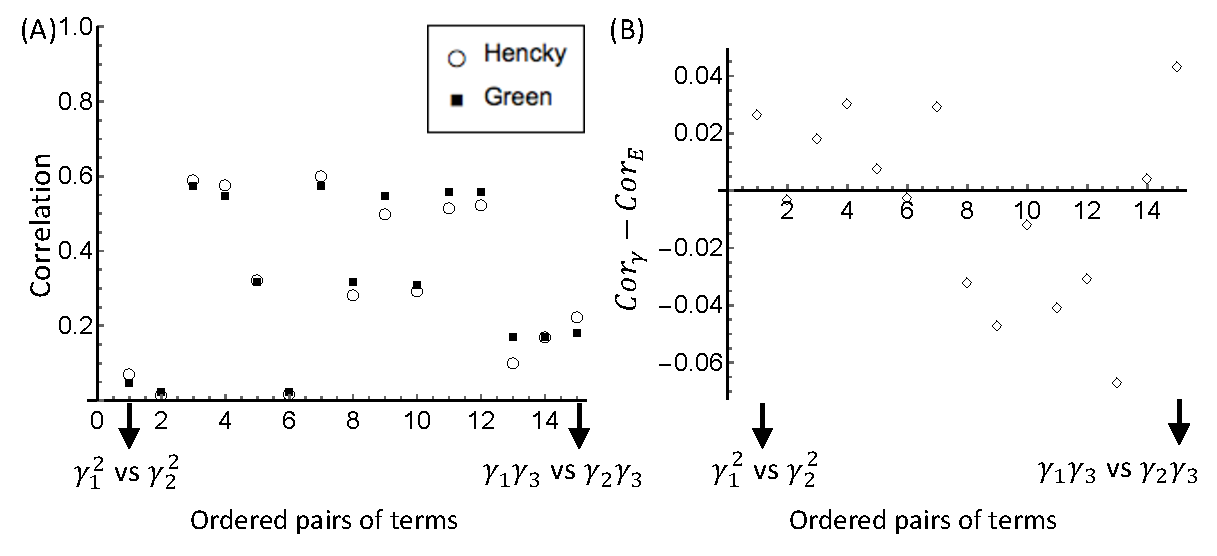
\includegraphics[width=\textwidth]{Images/chapter5/gvsecorrelation}
\caption{(A) The correlation between parameters pairs in the generalized Fung model when using Green-Lagrange vs Hencky strains. (B) The difference in correlation between each pair of parameters, which is very small but with the Hencky strains being lower overall.}
\label{fig:gvsecorrelation}
\end{figure}
%-------------------	 end FIGURE 	-------------------%
%%%%%%%%%%%%%%%%%%%%%%%%%%%%%%%%%%%%%%%%%%%%%%%%%%%%%%%%%%%%

    
    The last and most important difference between Green-Lagrange and Hencky strains is that they handle compression very differently. With the same model form, stresses increase exponentially under compression with Hencky strains, but only mildly with Green-Lagrange strains. We illustrated this again using the generalized Fung model (Eqn. \ref{eqn:generalizedfungmodel}) in the physiologically relevant range, with Green-Lagrange or Hencky strain as the input variable (Fig. \ref{fig:gvsecompression}). The reason for this is actually fairly simple, Green-Lagrange strain maps deformations from $\mathbf{E}: [0,\infty] \rightarrow [-1/2,\infty]$, while Hencky strains maps deformations from $\mathbf{\gamma}: [0,\infty] \rightarrow [-\infty,\infty]$, drastically increasing the magnitude of the same strain value under compression. This behavior very convenient for modeling collageneous tissues, where collagen fibers crimps unload compression but do not increase the stress \cite{soares_mathematical_2017}. Due to all factors considered (Table \ref{tb:greenvshencky}), we proceed to use the Green-Lagrange strain tensor as the best kinematic basis to formulate the effective constitutive model. 
    
    
%%%%%%%%%%%%%%%%%%%%%%%%%%%%%%%%%%%%%%%%%%%%%%%%%%%%%%%%%%%%
%-------------------	begin FIGURE 	-------------------%
\begin{figure}
\centering
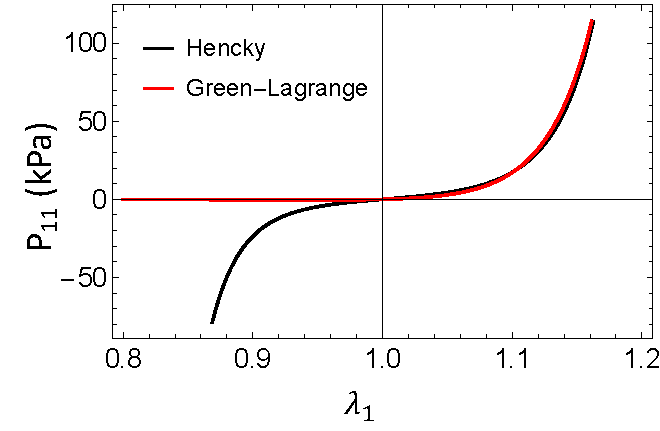
\includegraphics[width=3.25in]{Images/chapter5/gvsecompression}
\caption{The response of a generalized Fung model when using Green-Lagrange (Black) vs Hencky strains(Red). Both models are able to match extensional response nearly perfectly with respect to each other, but drastically differ in response under compression.}
\label{fig:gvsecompression}
\end{figure}
%-------------------	 end FIGURE 	-------------------%
%%%%%%%%%%%%%%%%%%%%%%%%%%%%%%%%%%%%%%%%%%%%%%%%%%%%%%%%%%%%


	





%----------------------------------------------------------%
%-------------------	begin TABLE 	-------------------%
\begin{table}
\caption{The difference between using the Green-Lagrange strain tensor versus the Hencky strains to formulate constitutive models. \textbf{Bold} text indicates key advantages and \textit{Italic} text indicate key disadvantages.}
\begin{center}
\label{tb:greenvshencky}
\begin{tabular}{|L{0.9in}|L{2.25in}|L{2.25in}|}
\hline
\rowcolor{Gray}
\multicolumn{1}{|c|}{Attributes} 
	& \multicolumn{1}{c|}{\textbf{Green-Lagrange strain}} 
    & \multicolumn{1}{c|}{\textbf{Hencky strain}}\\
\hline
General & Most commonly used in modeling	& \textbf{Easy to interpret physically} \\
\hline
Stress 	& Even simpler form for the 2nd Piola Kirchhoff stress \footnotesize
\begin{equation*}
\begin{aligned}
\mathbf{S} =& \dpd{\Psi}{E_m}\mathbf{m}_0\otimes\mathbf{m}_0 + \dpd{\Psi}{E_n}\mathbf{n}_0\otimes\mathbf{n}_0 \\&+ \frac{1}{2}\dpd{\Psi}{E_{\phi}}\left(\mathbf{m}_0\otimes\mathbf{n}_0+\mathbf{n}_0\otimes\mathbf{m}_0\right)
\end{aligned}
\end{equation*}
\normalsize
	& Simple form for the Cauchy stress	\footnotesize
\begin{equation*}
\begin{aligned}
\mathbf{T} =& \dpd{\Psi}{\gamma_{1}}\mathbf{m}_t\otimes\mathbf{m}_t + \dpd{\Psi}{\gamma_{2}}\mathbf{n}_t\otimes\mathbf{n}_t \\ &+ \frac{\lambda_n}{\lambda_m}\dpd{\Psi}{\gamma_{3}}\left(\mathbf{m}_t\otimes\mathbf{n}_t+\mathbf{n}_t\otimes\mathbf{m}_t\right)
\end{aligned}
\end{equation*}
\normalsize
\\
\hline
Elasticity tensor & \textbf{Much simpler form for the elasticity tensor}
	& \textit{The equations for the elasticity tensor is extremely long} \\
\hline
Parameter covariance 	& 	& \textbf{Modestly less correlation between parameters} \\
\hline
Response under compression	&	\textbf{Modest changes in stress under compression, behaves much more similar to soft tissues due to collagen fiber crimp}
	& \textit{Behaves badly under large compression} \begin{itemize}
	\item Log scaling cause the strain energy to increase exponentially with compression
	\end{itemize}\\
\hline
\end{tabular}
\end{center}
\end{table}
%-------------------	 end TABLE 		-------------------%
%----------------------------------------------------------%

%---    METHODS
\section{Elasticity tensor}\label{sec:elasticitytensor}

	An analytical form for the elasticity tensor is extremely important for fast and convergent numerical simulations. A constitutive model without a smooth, continuous, and convex elasticity tensor can pose significant problems for simulation of nonlinear materials to converge quickly, or even to converge at all. The strain basis used for the model can have significant impact on the form of the elasticity tensor. Here, we derived the generalized form of the elasticity tensor for using the Green-Lagrange basis (Eqn. \ref{eqn:greenstrain}) and the Hencky strain basis (Eqn. \ref{eqn:henckystrains}). Note that this is the generalized form, which does not depend on the explicit form of the constitutive model, it is only a function of the strain basis and the response functions (derivatives of the strain energy function), whose form doesn't not have to be explicitly stated. The 9 response functions are:
%=======	BEGIN Equation		=======%
\begin{equation}
\dpd{\Psi}{E_m}, \quad \dpd{\Psi}{E_n}, \quad \dpd{\Psi}{E_\phi}, \quad \frac{\partial^2\Psi}{\partial E_m^2}, \quad \frac{\partial^2\Psi}{\partial E_n^2}, \quad \frac{\partial^2\Psi}{\partial E_\phi^2}, \quad \frac{\partial^2\Psi}{\partial E_m\partial E_n}, \quad \frac{\partial^2\Psi}{\partial E_m\partial E_\phi}, \quad \frac{\partial^2\Psi}{\partial E_n\partial E_\phi}.
\end{equation}
%=======	END Equation		=======%
    
\subsection{Derivation with Green-Lagrange strain}
	
    The elasticity tensor is given by the second derivative of the strain energy function with respect to the right Cauchy strain. Using the chain rules, fully expanding all terms, and enforcing symmetry of partial derivatives, $\md{\Psi}{2}{E_m}{}{E_n}{} = \md{\Psi}{2}{E_n}{}{E_m}{}$, the generalized form for the elasticity tensor is given by 
%=======	BEGIN Equation		=======%
\begin{equation} \label{eqn:generalizedelasticityform}
\begin{aligned}
\dod[2]{\Psi}{\mathbf{C}} =& 
	\dpd{\Psi}{E_m} \dod[2]{E_m}{\mathbf{C}} 
    + \dpd{\Psi}{E_n} \dod[2]{E_n}{\mathbf{C}}
    + \dpd{\Psi}{E_\phi} \dod[2]{E_\phi}{\mathbf{C}} \\
+& \dpd[2]{\Psi}{E_m} \dod{E_m}{\mathbf{C}}\dod{E_m}{\mathbf{C}} 
	+ \dpd[2]{\Psi}{E_n} \dod{E_n}{\mathbf{C}} \dod{E_n}{\mathbf{C}} 
    + \dpd{\Psi}{E_\phi} \dod{E_\phi}{\mathbf{C}} \dod{E_\phi}{\mathbf{C}} \\
+& \dmd{\Psi}{2}{E_m}{}{E_n}{} \left(\dod{E_n}{\mathbf{C}} \dod{E_m}{\mathbf{C}} + \dod{E_m}{\mathbf{C}} \dod{E_n}{\mathbf{C}}\right)   \\
    +& \dmd{\Psi}{2}{E_m}{}{E_\phi}{} \left(\dod{E_\phi}{\mathbf{C}} \dod{E_m}{\mathbf{C}} + \dod{E_m}{\mathbf{C}} \dod{E_\phi}{\mathbf{C}}\right)  \\
    +& \dmd{\Psi}{2}{E_n}{}{E_\phi}{} \left(\dod{E_n}{\mathbf{C}} \dod{E_\phi}{\mathbf{C}} + \dod{E_\phi}{\mathbf{C}} \dod{E_n}{\mathbf{C}}\right).  \\
\end{aligned}
\end{equation}
%=======	END Equation		=======%
To break this down, we begin with the derivatives of the Green-Lagrange strains, which are given by,
%==========================================================%
%-------------------	begin EQUATION 	-------------------%
\begin{equation}\label{eqn:partialgreens}
\begin{aligned}
\dod{E_m}{\mathbf{C}} &= \frac{1}{2} \mathbf{m}\otimes\mathbf{m}	\\
\dod{E_n}{\mathbf{C}} &= \frac{1}{2} \mathbf{n}\otimes\mathbf{n} \\
\dod{E_\phi}{\mathbf{C}} &= \frac{1}{4} \left(\mathbf{m}\otimes\mathbf{n} + \mathbf{n}\otimes\mathbf{m} \right),
\end{aligned}
\end{equation}
%-------------------	 end EQUATION 	-------------------%
%==========================================================%
and 
%==========================================================%
%-------------------	begin EQUATION 	-------------------%
\begin{equation}
\dod[2]{E_m}{\mathbf{C}} = \dod[2]{E_n}{\mathbf{C}} = \dod[2]{E_\phi}{\mathbf{C}} = \mathbf{0}.
\end{equation}
%-------------------	 end EQUATION 	-------------------%
%==========================================================%
Right away, the Green-Lagrange strains have the benefit of the second derivatives being zero, reducing the elasticity tensor (Eqn. \ref{eqn:generalizedelasticityform}) from 9 to 6 terms. Substituting with the partial derivatives (Eqn. \ref{eqn:partialgreens}) gives
%==========================================================%
%-------------------	begin EQUATION 	-------------------%
\begin{equation}\label{eqn:greenelasticityform}
\begin{aligned}
\dod[2]{\Psi}{\mathbf{C}} =
	& \frac{1}{4}\dpd[2]{\Psi}{E_m} \mathbf{m}\otimes\mathbf{m}\otimes\mathbf{m}\otimes\mathbf{m}	\\
    &+ \frac{1}{8}\dmd{\Psi}{2}{E_m}{}{E_\phi}{} 
    	\left(
        	\mathbf{m}\otimes\mathbf{m}\otimes\mathbf{m}\otimes\mathbf{n}
            +\mathbf{m}\otimes\mathbf{m}\otimes\mathbf{n}\otimes\mathbf{m} \right.\\
            &\quad +\left.\mathbf{m}\otimes\mathbf{n}\otimes\mathbf{m}\otimes\mathbf{m}
            +\mathbf{n}\otimes\mathbf{m}\otimes\mathbf{m}\otimes\mathbf{m}
        \right)	\\
    &+ \frac{1}{4}\dmd{\Psi}{2}{E_m}{}{E_n}{} 
    	\left(
        	\mathbf{m}\otimes\mathbf{m}\otimes\mathbf{n}\otimes\mathbf{n}
            +\mathbf{n}\otimes\mathbf{n}\otimes\mathbf{m}\otimes\mathbf{m}
        \right)	\\
    &+ \frac{1}{16}\dpd[2]{\Psi}{E_\phi} 
    	\left(
        	\mathbf{m}\otimes\mathbf{n}\otimes\mathbf{m}\otimes\mathbf{n}
            +\mathbf{m}\otimes\mathbf{n}\otimes\mathbf{n}\otimes\mathbf{m} \right. \\
            &\quad \left.+\mathbf{n}\otimes\mathbf{m}\otimes\mathbf{m}\otimes\mathbf{n}
            +\mathbf{n}\otimes\mathbf{m}\otimes\mathbf{n}\otimes\mathbf{m}
        \right)	\\
    &+ \frac{1}{8}\dmd{\Psi}{2}{E_n}{}{E_\phi}{} 
    	\left(
        	\mathbf{m}\otimes\mathbf{n}\otimes\mathbf{n}\otimes\mathbf{n}
            +\mathbf{n}\otimes\mathbf{m}\otimes\mathbf{n}\otimes\mathbf{n} \right. \\
            &\quad +\left. \mathbf{n}\otimes\mathbf{n}\otimes\mathbf{m}\otimes\mathbf{n}
            +\mathbf{n}\otimes\mathbf{n}\otimes\mathbf{n}\otimes\mathbf{m}
        \right)	\\
    &+ \frac{1}{4} \dpd[2]{\Psi}{E_n} \mathbf{n}\otimes\mathbf{n}\otimes\mathbf{n}\otimes\mathbf{n}	\\
\end{aligned}
\end{equation}
%-------------------	 end EQUATION 	-------------------%
%==========================================================%


\subsection{Derivation with Hencky strains}

	The elasticity tensor when using the Hencky strains is much more complex. For start, the second derivatives of the Hencky strains are non-zero. The derivatives themselves are complex both in form and conceptually. The derivation of the derivatives is not straight forward. To make this simpler, we start with an alternative definition for the Hencky strains, which relates the 4 variables, $\gamma_1$, $\gamma_2$, $\gamma_3$, and $\mathbf{C}$.  
%==========================================================%
%-------------------	begin EQUATION 	-------------------%
\begin{equation}\label{eqn:invariantset}
\begin{aligned}
    \gamma_1 &= \ln \left( \lambda_m \right), &  \lambda_m^2 &= \mathbf{m}\cdot\mathbf{C}\mathbf{m}  \\
    \gamma_2 &= \ln \left( \lambda_n \right), &  \lambda_n^2 &= \mathbf{n}\cdot\mathbf{C}\mathbf{n} 
                    - \lambda_m^2 \phi^2   \\
    \gamma_3 &= \phi, & \phi &= \left( \lambda_m\right)^{-2}\mathbf{m}\cdot\mathbf{C}\mathbf{n}.
\end{aligned}
\end{equation}
%-------------------	 end EQUATION 	-------------------%
%==========================================================%
It is important here that with this definition, the vector basis, $\mathbf{m}$ and $\mathbf{n}$, are defined on the reference coordinate system, which does not change with deformation. By chain rule, the first derivatives are as followed,
%==========================================================%
%-------------------	begin EQUATION 	-------------------%
\begin{subequations}
\begin{align}
\dod{\gamma_1}{\mathbf{C}} =& \dpd{\gamma_1}{\lambda_m}\dod{\lambda_m}{\mathbf{C}},	
	& \dod{\lambda_m^2}{\mathbf{C}} =& \dpd{\lambda_m^2}{\mathbf{C}}:\dod{\mathbf{C}}{\mathbf{C}} 
	+ \dpd{\lambda_m^2}{\lambda_n}\dod{\lambda_n}{\mathbf{C}}
    + \dpd{\lambda_m^2}{\phi}\dod{\phi}{\mathbf{C}} \\
\dod{\gamma_2}{\mathbf{C}} =& \dpd{\gamma_2}{\lambda_n}\dod{\lambda_n}{\mathbf{C}},	
	& \dod{\lambda_n^2}{\mathbf{C}} =& \dpd{\lambda_n^2}{\mathbf{C}}:\dod{\mathbf{C}}{\mathbf{C}} 
	+ \dpd{\lambda_n^2}{\lambda_m}\dod{\lambda_m}{\mathbf{C}}
    + \dpd{\lambda_n^2}{\phi}\dod{\phi}{\mathbf{C}} \\
\dod{\gamma_3}{\mathbf{C}} =& \dod{\phi}{\mathbf{C}},
	& \dod{\phi}{\mathbf{C}} =& \dpd{\phi}{\mathbf{C}}:\dod{\mathbf{C}}{\mathbf{C}} 
	+ \dpd{\phi}{\lambda_m}\dod{\lambda_m}{\mathbf{C}}
    + \dpd{\phi}{\lambda_n}\dod{\lambda_n}{\mathbf{C}}. 
\end{align}
\end{subequations}
%-------------------	 end EQUATION 	-------------------%
%==========================================================%
First, note that all the partial derivatives are functions of each other. This is indeed problematic, but also note from equation \ref{eqn:invariantset} that $\lambda_m$ does not depend on $\lambda_n$ and $\phi$, and $\phi$ does not depend on $\lambda_n$. This means that the following partial derivatives are zero,
%==========================================================%
%-------------------	begin EQUATION 	-------------------%
\begin{equation}\label{eqn:henckystraindependence}
\begin{aligned}
\dpd{\lambda_m}{\lambda_n} = \dpd{\lambda_m}{\phi} = \dpd{\phi}{\lambda_n} = 0,
\end{aligned}
\end{equation}
%-------------------	 end EQUATION 	-------------------%
%==========================================================%
allowing the equations to be solved. 

	For the second derivatives, note from the definition we have above, the Hencky strains are only linear function of $\mathbf{C}$, thus their 2nd \emph{partial derivatives} are zero with respect to $\mathbf{C}$ only,
%==========================================================%
%-------------------	begin EQUATION 	-------------------%
\begin{equation}
\begin{aligned}
\dpd{}{\mathbf{C}}\left(\dod{\gamma_1}{\mathbf{C}}\right) 
	=\dpd{}{\mathbf{C}}\left(\dod{\gamma_2}{\mathbf{C}}\right)
    =\dpd{}{\mathbf{C}}\left(\dod{\gamma_3}{\mathbf{C}}\right)
    =0.
\end{aligned}
\end{equation}
%-------------------	 end EQUATION 	-------------------%
%==========================================================%
The second derivatives are thus defined to be,
%==========================================================%
%-------------------	begin EQUATION 	-------------------%
\begin{subequations}
\begin{align}
\dod{}{\mathbf{C}}\left(\dod{\gamma_1}{\mathbf{C}}\right) =&
    \dpd{}{\lambda_m}\left(\dod{\gamma_1}{\mathbf{C}}\right)\dod{\lambda_m}{\mathbf{C}}
    + \dpd{}{\lambda_n}\left(\dod{\gamma_1}{\mathbf{C}}\right)\dod{\lambda_n}{\mathbf{C}}
    + \dpd{}{\phi}\left(\dod{\gamma_1}{\mathbf{C}}\right)\dod{\phi}{\mathbf{C}}	\\
\dod{}{\mathbf{C}}\left(\dod{\gamma_2}{\mathbf{C}}\right) =&
    \dpd{}{\lambda_m}\left(\dod{\gamma_2}{\mathbf{C}}\right)\dod{\lambda_m}{\mathbf{C}}
    + \dpd{}{\lambda_n}\left(\dod{\gamma_2}{\mathbf{C}}\right)\dod{\lambda_n}{\mathbf{C}}
    + \dpd{}{\phi}\left(\dod{\gamma_2}{\mathbf{C}}\right)\dod{\phi}{\mathbf{C}}	\\
\dod{}{\mathbf{C}}\left(\dod{\phi}{\mathbf{C}}\right) =&
    \dpd{}{\lambda_m}\left(\dod{\phi}{\mathbf{C}}\right)\dod{\lambda_m}{\mathbf{C}}
    + \dpd{}{\lambda_n}\left(\dod{\phi}{\mathbf{C}}\right)\dod{\lambda_n}{\mathbf{C}}
    + \dpd{}{\phi}\left(\dod{\phi}{\mathbf{C}}\right)\dod{\phi}{\mathbf{C}} 
\end{align}
\end{subequations}
%-------------------	 end EQUATION 	-------------------%
%==========================================================%
Taking advantage of equation \ref{eqn:henckystraindependence}, the first and second derivatives of the Hencky strains are presented as followed:
%==========================================================%
%-------------------	begin EQUATION 	-------------------%
\begin{subequations} \label{eqn:henckyderivatives}
\begin{align}
\dod{\gamma_1}{\mathbf{C}} =& \frac{1}{2\lambda_m^2} \mathbf{m}\otimes\mathbf{m}	\\
\dod{\gamma_2}{\mathbf{C}} =& \frac{1}{2\lambda_n^2} \left(\mathbf{n}\otimes\mathbf{n} - \phi \left( \mathbf{m}\otimes\mathbf{n} + \mathbf{n}\otimes\mathbf{m}\right) + \phi^2 \mathbf{m}\otimes\mathbf{m} \right)	\\
\dod{\gamma_3}{\mathbf{C}} =& \frac{1}{2\lambda_m^2} \left( \mathbf{m}\otimes\mathbf{n} + \mathbf{n}\otimes\mathbf{m} - 2\phi \mathbf{m}\otimes\mathbf{m}\right) \\
\dod[2]{\gamma_1}{\mathbf{C}} =& -\frac{1}{2}\frac{1}{\lambda_m^4}\mathbf{m}\otimes\mathbf{m} \otimes \mathbf{m}\otimes\mathbf{m}	\\
\begin{split}
\dod[2]{\gamma_2}{\mathbf{C}} =& -\frac{1}{2}\frac{1}{\lambda_n^4} 
    \left[
    \mathbf{n}\otimes\mathbf{n}\otimes\mathbf{n}\otimes\mathbf{n}
    -\phi \mathbf{m}\otimes\mathbf{n}\otimes\mathbf{n}\otimes\mathbf{n}
    -\phi \mathbf{n}\otimes\mathbf{m}\otimes\mathbf{n}\otimes\mathbf{n}\right.   \\
    &-\phi \mathbf{n}\otimes\mathbf{n}\otimes\mathbf{m}\otimes\mathbf{n}
    -\phi \mathbf{n}\otimes\mathbf{n}\otimes\mathbf{n}\otimes\mathbf{m}   
    +\phi^2 \mathbf{m}\otimes\mathbf{m}\otimes\mathbf{n}\otimes\mathbf{n} \\
    &\left.+\phi^2 \mathbf{n}\otimes\mathbf{n}\otimes\mathbf{m}\otimes\mathbf{m}
    \right]\\
    &-\left(\frac{1}{4}\frac{1}{\lambda_m^2\lambda_n^2} + \frac{1}{2}\phi^2\frac{1}{\lambda_n^4} \right)
    \left[
    \mathbf{m}\otimes\mathbf{n}\otimes\mathbf{m}\otimes\mathbf{n}
    +\mathbf{m}\otimes\mathbf{n}\otimes\mathbf{n}\otimes\mathbf{m} \right. \\
    &+\left. \mathbf{n}\otimes\mathbf{m}\otimes\mathbf{m}\otimes\mathbf{n}
    +\mathbf{n}\otimes\mathbf{m}\otimes\mathbf{n}\otimes\mathbf{m}
    \right]\\
    &+\left(\frac{1}{2}\phi\frac{1}{\lambda_m^2\lambda_n^2} + \frac{1}{2}\phi^3\frac{1}{\lambda_n^4} \right)
    \left[
    \mathbf{m}\otimes\mathbf{m}\otimes\mathbf{m}\otimes\mathbf{n}
    +\mathbf{m}\otimes\mathbf{m}\otimes\mathbf{n}\otimes\mathbf{m} \right. \\
    &+\left. \mathbf{m}\otimes\mathbf{n}\otimes\mathbf{m}\otimes\mathbf{m}
    +\mathbf{n}\otimes\mathbf{m}\otimes\mathbf{m}\otimes\mathbf{m}
    \right]\\
    &-\left(\phi^2\frac{1}{\lambda_m^2\lambda_n^2} + \frac{1}{2}\phi^4\frac{1}{\lambda_n^4} \right)
    \left[
    \mathbf{m}\otimes\mathbf{m}\otimes\mathbf{m}\otimes\mathbf{m}
    \right]
\end{split}\\
\begin{split}
\dod[2]{\gamma_3}{\mathbf{C}} =& -\frac{1}{2}\frac{1}{\lambda_m^4} \times \left(
        \mathbf{n}\otimes\mathbf{m}\otimes\mathbf{m}\otimes\mathbf{m} + \mathbf{m}\otimes\mathbf{n}\otimes\mathbf{m}\otimes\mathbf{m}\right. \\
        &+ \left.\mathbf{m}\otimes\mathbf{m}\otimes\mathbf{n}\otimes\mathbf{m} +
        \mathbf{m}\otimes\mathbf{m}\otimes\mathbf{m}\otimes\mathbf{n} - 
        4\phi\mathbf{m}\otimes\mathbf{m} \otimes \mathbf{m}\otimes\mathbf{m} \right)
\end{split}
\end{align}
\end{subequations}
%-------------------	 end EQUATION 	-------------------%
%==========================================================%

	Saving everyone from the algebra, without further ado, the most elegant form of the elasticity tensor for constitutive models based on the Hencky strains is, 
%==========================================================%
%-------------------	begin EQUATION 	-------------------%
\begin{subequations} \label{eqn:elasticityhencky}
\begin{align}
\begin{split}
\dod[2]{\Psi}{\mathbf{C}} =&
	\psi_1 \mathbf{m}\otimes\mathbf{m}\otimes\mathbf{m}\otimes\mathbf{m}	\\
    &+ \psi_2
    	\left(
        	\mathbf{m}\otimes\mathbf{m}\otimes\mathbf{m}\otimes\mathbf{n}
            +\mathbf{m}\otimes\mathbf{m}\otimes\mathbf{n}\otimes\mathbf{m} \right. \\
            &\quad +\left. \mathbf{m}\otimes\mathbf{n}\otimes\mathbf{m}\otimes\mathbf{m}
            +\mathbf{n}\otimes\mathbf{m}\otimes\mathbf{m}\otimes\mathbf{m}
        \right)	\\
    &+ \psi_3
    	\left(
        	\mathbf{m}\otimes\mathbf{m}\otimes\mathbf{n}\otimes\mathbf{n}
            +\mathbf{n}\otimes\mathbf{n}\otimes\mathbf{m}\otimes\mathbf{m}
        \right)	\\
    &+ \psi_4
    	\left(
        	\mathbf{m}\otimes\mathbf{n}\otimes\mathbf{m}\otimes\mathbf{n}
            +\mathbf{m}\otimes\mathbf{n}\otimes\mathbf{n}\otimes\mathbf{m} \right. \\
            &\quad +\left.\mathbf{n}\otimes\mathbf{m}\otimes\mathbf{m}\otimes\mathbf{n}
            +\mathbf{n}\otimes\mathbf{m}\otimes\mathbf{n}\otimes\mathbf{m}
        \right)	\\
    &+ \psi_5
    	\left(
        	\mathbf{m}\otimes\mathbf{n}\otimes\mathbf{n}\otimes\mathbf{n}
            +\mathbf{n}\otimes\mathbf{m}\otimes\mathbf{n}\otimes\mathbf{n}
            +\mathbf{n}\otimes\mathbf{n}\otimes\mathbf{m}\otimes\mathbf{n}
            +\mathbf{n}\otimes\mathbf{n}\otimes\mathbf{n}\otimes\mathbf{m}
        \right)	\\
    &+ \psi_6 \mathbf{n}\otimes\mathbf{n}\otimes\mathbf{n}\otimes\mathbf{n}
\end{split}	\\
\begin{split}
\psi_1 =&
        -\frac{1}{2}\frac{1}{\lambda_m^4}W^{(1)}
        -\left(\frac{\phi^2}{\lambda_m^2\lambda_n^2}+\frac{1}{2}\frac{\phi^4}{\lambda_n^4}\right)W^{(2)}
        +2\frac{\phi}{\lambda_m^4}W^{(3)}
        +\frac{1}{4}\frac{1}{\lambda_m^4}W^{(11)}   \\
        &+\frac{1}{4}\frac{\phi^4}{\lambda_n^4}W^{(22)}
        +\frac{\phi^2}{\lambda_m^4}W^{(33)}
        +\frac{1}{2}\frac{\phi^2}{\lambda_m^2\lambda_n^2}W^{(12)}
        -\frac{\phi}{\lambda_m^4}W^{(13)}
        -\frac{\phi^3}{\lambda_m^2 \lambda_n^2}W^{(23)}
\end{split}	\\
\begin{split}
\psi_2 =&
        \frac{1}{2}\left(\frac{\phi}{\lambda_m^2\lambda_n^2} + \frac{\phi^3}{\lambda_n^4}\right)W^{(2)}
        -\frac{1}{2}\frac{1}{\lambda_m^4}W^{(3)}
        -\frac{1}{4}\frac{\phi^3}{\lambda_n^4}W^{(22)}
        -\frac{1}{2}\frac{\phi}{\lambda_m^4}W^{(33)}    \\
        &-\frac{1}{4}\frac{\phi}{\lambda_m^2 \lambda_n^2}W^{(12)}
        +\frac{1}{4}\frac{1}{\lambda_m^4}W^{(13)}
        +\frac{3}{4}\frac{\phi^2}{\lambda_m^2 \lambda_n^2}W^{(23)}
\end{split}	\\
\psi_3 =&
        -\frac{1}{2}\frac{\phi^2}{\lambda_n^4}W^{(2)}
        +\frac{1}{4}\frac{\phi^2}{\lambda_n^4}W^{(22)}
        +\frac{1}{4}\frac{1}{\lambda_m^2 \lambda_n^2}W^{(12)}
        -\frac{1}{2}\frac{\phi}{\lambda_m^2 \lambda_n^2}W^{(23)}	\\
\psi_4 =&
        -\left(\frac{1}{4}\frac{1}{\lambda_m^2\lambda_n^2}+\frac{1}{2}\frac{\phi^2}{\lambda_n^4}\right)W^{(2)}
        +\frac{1}{4}\frac{\phi^2}{\lambda_n^4}W^{(22)}
        +\frac{1}{4}\frac{1}{\lambda_m^4}W^{(33)}
        -\frac{1}{2}\frac{\phi}{\lambda_m^2 \lambda_n^2}W^{(23)}	\\
\psi_5 =&
        \frac{1}{2}\frac{\phi}{\lambda_n^4}W^{(2)}
        -\frac{1}{4}\frac{\phi}{\lambda_n^4}W^{(22)}
        +\frac{1}{4}\frac{1}{\lambda_m^2 \lambda_n^2}W^{(23)}	\\
\psi_6 =&
        -\frac{1}{2}\frac{1}{\lambda_n^4}W^{(2)}
        +\frac{1}{4}\frac{1}{\lambda_n^4}W^{(22)}
\end{align}
\end{subequations}
%-------------------	 end EQUATION 	-------------------%
%==========================================================%
where $W^{ij} = \md{\Psi}{2}{\gamma_i}{}{\gamma_j}{}$.

\paragraph{Some final remarks} 
	The elasticity tensor for the Hencky strains (Eqn. \ref{eqn:elasticityhencky}) are somewhat complicated, but most terms are weighted by $\gamma_3$, which is the shear angle $\phi$. Under no shear, the form for the elasticity tensor reduces significantly, to similar in form to the Green-Lagrange strains (Eqn. \ref{eqn:greenelasticityform}). The shear angle is typically a small value as well, making most terms in the elasticity tensor small as well. However, they are still necessary to accurately compute the elasticity tensor and are representative of the coupling between the strains components. 
    
    More interesting is perhaps that the Hencky strains overall leads to less covariance in model parameters overall, despite there being many more coupling terms than the Green-Lagrange strain. This is indicative of the covariance within the model form and of the tissue, which in turn is necessary to reproduce soft tissue responses. Due to this natural covariance of the tissues themselves, truly non-covariant models are not feasibly attainable. The level of covariance demonstrated by $\Psi_{eff}$ (Eqn. \ref{eqn:finalexponentialmodelformscaled}) within are likely close to optimal without sacrificing for addition model complexity. 



















% loss of benefits for the correlation between parameters from polynomial to exponential model. 

%---    Results
\section{Parameter correlation}\label{sec:parametercorrelation}

	The Fisher's information matrix for a maximum likelihood problem described by a multivariate normally distributed statistical model is defined to be the negative of the second partial derivatives of the log-likelihood function with respect to the parameters, $\xi_i$, evaluated at the maximum likelihood estimates. When converting to least squares minimization, which is equivalent of a negative log-likelihood minimization, the information matrix is defined to be
%==========================================================%
%-------------------	begin EQUATION 	-------------------%
\begin{equation}\label{eqn:informationmatrix}
\begin{aligned}
\mathcal{I}_{jk} = \dmd{\mathcal{F}}{2}{\xi_j}{}{\xi_k}{} = \mathcal{H}_{jk},
\end{aligned}
\end{equation}
%-------------------	 end EQUATION 	-------------------%
%==========================================================%
which is also exactly the Hessian matrix, $\mathbfcal{H}$, at the best fit value. The D-optimality is the determinant of this information matrix, whereas other optimality measures are mostly similar functions of this information matrix. The main reason is because, for a maximum likelihood problem governed by a normally distributed statistical model, the covariance matrix is exactly proportional to the inverse of the information matrix,
%==========================================================%
%-------------------	begin EQUATION 	-------------------%
\begin{equation}\label{eqn:covariancematrix}
\begin{aligned}
\mathbf{Cov} = \sigma^2 \mathbfcal{I}^{-1},
\end{aligned}
\end{equation}
%-------------------	 end EQUATION 	-------------------%
%==========================================================%
where $\sigma^2$ is the scalar variance of the statistical model, and can be estimated by the mean squared error weighted by the degree of freedom. Maximizing the D-optimality is equivalent of minimizing the variance of each parameter along with minimizing the covariance between parameters. Defining the objective function as
%==========================================================%
%-------------------	begin EQUATION 	-------------------%
\begin{equation}
\begin{aligned}
\mathcal{F} = \sum_i \left(f(x_i) - f_i\right)^2,
\end{aligned}
\end{equation}
%-------------------	 end EQUATION 	-------------------%
%----------------------------------------------------------%
where $f(x_i)$ is the model and $f_i$ are date points, the information matrix, or Hessian matrix, is given by 
%==========================================================%
%-------------------	begin EQUATION 	-------------------%
\begin{equation}\label{eqn:hessianmatrix}
\begin{aligned}
\dpd{\mathcal{F}}{\xi_j} =& \sum_i 2\left(f(x_i) - f_i\right)\dpd{f(x_i)}{\xi_j}	\\
\mathcal{H}_{jk} = \dmd{\mathcal{F}}{2}{\xi_j}{}{\xi_k}{} =& \sum_i 2\dpd{f(x_i)}{\xi_k}\dpd{f(x_i)}{\xi_j}	+ 2\left(f(x_i) - f_i\right)\dmd{f(x_i)}{2}{\xi_j}{}{\xi_k}{}
\end{aligned}
\end{equation}
%-------------------	 end EQUATION 	-------------------%
%----------------------------------------------------------%
Note here that $\mathcal{J}_{ij} = \dpd{f(x_i)}{\xi_j}$ is the Jacobian matrix for the non-linear least squares problem, and when the errors are small, i.e. when the model fits the data, in other words such that $\left(f(x_i) - f_i\right)$ is small or approximately 0, then the information matrix can by approximated by  
\begin{equation}
\mathcal{I}_{jk} \approx \mathcal{J}_{ji}\mathcal{J}_{ik} \quad \mathrm{or} \quad
\mathbfcal{I} \approx \mathbfcal{J}^\mathsf{T}\mathbfcal{J},
\end{equation}
a form much more familiar to most doing nonlinear least squares parameter estimation. 


	For $\Psi_{eff}$ (Eqn. \ref{eqn:finalexponentialmodelformscaled}), let $f = c_0Q^\prime e^{Q}$ be the stress, where $Q^\prime$ is one of $\pd{Q}{E_m}$, $\pd{Q}{E_n}$, or $\pd{Q}{E_\phi}$. The Jacobian matrix is thus, 
\begin{equation}	
\mathcal{J}_{ij} = Q^\prime e^Q \delta_{0j} + c_0 e^Q \dpd{Q^\prime}{\xi_j}+ c_0Q^\prime e^Q \dpd{Q}{\xi_j}
\end{equation}
Note that since $Q$ is a sum of polynomials, the second partial derivatives of $Q$ and $Q^\prime$ with respect to $\mathbf{\xi}$ is precisely 0,
\begin{equation}		
\md{Q}{2}{\xi_j}{}{\xi_k}{}  = \md{Q^\prime}{2}{\xi_j}{}{\xi_k}{} = 0.
\end{equation}
Thus,
\begin{equation}	
\begin{aligned}
\dmd{f}{2}{\xi_j}{}{\xi_k}{} =& e^Q \delta_{0j}\dpd{Q^\prime}{\xi_k} + Q^\prime e^Q \delta_{0j}\dpd{Q}{\xi_k} 
+  e^Q\dpd{Q^\prime}{\xi_j}\delta_{0k} + c_0 e^Q\dpd{Q^\prime}{\xi_j}\dpd{Q}{\xi_k} 
+ Q^\prime e^Q \dpd{Q}{\xi_j}\delta_{0k} 	\\
&+ c_0e^Q \dpd{Q}{\xi_j}\dpd{Q^\prime}{\xi_k}
+ c_0Q^\prime e^Q \dpd{Q}{\xi_j}\dpd{Q}{\xi_k} 
\end{aligned}
\end{equation}
and the Hessian matrix is given by
% \begin{equation}	
% \begin{aligned}
% \mathcal{H}_{jk} &= 2\sum_i\left[ (Q^\prime e^Q)^2  \delta_{0j}\delta_{0k} + c_0Q^\prime e^{2Q} \delta_{0j}\dpd{Q^\prime}{\xi_k}+ c_0 (Q^\prime e^Q)^2 \delta_{0j}\dpd{Q}{\xi_k}\right.	\\
% &+c_0Q^\prime e^{2Q} \dpd{Q^\prime}{\xi_j} \delta_{0k} + (c_0 e^Q)^2 \dpd{Q^\prime}{\xi_j}\dpd{Q^\prime}{\xi_k}+ (c_0e^Q)^2Q^\prime  \dpd{Q^\prime}{\xi_j}\dpd{Q}{\xi_k}	\\
% &+ c_0(Q^\prime e^Q)^2 \dpd{Q}{\xi_j}\delta_{0k} + Q^\prime (c_0 e^Q)^2 \dpd{Q}{\xi_j}\dpd{Q^\prime}{\xi_k}+ (c_0Q^\prime e^Q)^2 \dpd{Q}{\xi_j}\dpd{Q}{\xi_k}	\\
% &+ (c_0Q^\prime e^Q - f_i)\left( e^Q \delta_{0j}\dpd{Q^\prime}{\xi_k} + Q^\prime e^Q \delta_{0j}\dpd{Q}{\xi_k} 
% +  e^Q\dpd{Q^\prime}{\xi_j}\delta_{0k} 
% \right.	\\
% &\left.\left.+ c_0 e^Q\dpd{Q^\prime}{\xi_j}\dpd{Q}{\xi_k} + Q^\prime e^Q \dpd{Q}{\xi_j}\delta_{0k}  + c_0e^Q \dpd{Q}{\xi_j}\dpd{Q^\prime}{\xi_k}
% + c_0Q^\prime e^Q \dpd{Q}{\xi_j}\dpd{Q}{\xi_k} \right)\right]
% \end{aligned}
% \end{equation}

\begin{equation}	
\begin{aligned}
\mathcal{H}_{jk} &= 2\sum_i\left[ (Q^\prime e^Q)^2  \delta_{0j}\delta_{0k} + c_0Q^\prime e^{2Q} \left(\delta_{0j}\dpd{Q^\prime}{\xi_k} + \dpd{Q^\prime}{\xi_j} \delta_{0k}\right) \right.	\\
&+ c_0 (Q^\prime e^Q)^2 \left(\delta_{0j}\dpd{Q}{\xi_k} + \dpd{Q}{\xi_j}\delta_{0k}\right) + (c_0 e^Q)^2 \dpd{Q^\prime}{\xi_j}\dpd{Q^\prime}{\xi_k} \\
&+  (c_0e^Q)^2Q^\prime \left( \dpd{Q^\prime}{\xi_j}\dpd{Q}{\xi_k}	+ \dpd{Q}{\xi_j}\dpd{Q^\prime}{\xi_k}\right) + (c_0Q^\prime e^Q)^2 \dpd{Q}{\xi_j}\dpd{Q}{\xi_k} \\
&+ (c_0Q^\prime e^Q - f_i)\left.\left[ e^Q \left(\delta_{0j}\dpd{Q^\prime}{\xi_k} + \dpd{Q^\prime}{\xi_j}\delta_{0k}\right) + Q^\prime e^Q \left(\delta_{0j}\dpd{Q}{\xi_k}  + \dpd{Q}{\xi_j}\delta_{0k}\right)
\right.\right.	\\
&\left.\left.+ c_0 e^Q\left(\dpd{Q^\prime}{\xi_j}\dpd{Q}{\xi_k}  +  \dpd{Q}{\xi_j}\dpd{Q^\prime}{\xi_k}\right)
+ c_0Q^\prime e^Q \dpd{Q}{\xi_j}\dpd{Q}{\xi_k} \right]\right].
\end{aligned}
\end{equation}
Here, the summation is over each data point $i$ and then sums for each component of stress $S_m$, $S_n$, and $S_\phi$ for $Q^\prime = \pd{Q}{E_m}$, $\pd{Q}{E_n}$ and $\pd{Q}{E_\phi}$ respectively. 

	Using this approach, we compared the covariance of the model parameters for with Green-Lagrange strains and with Hencky strains for the Fung model (Table \ref{tb:correlationE}\&\ref{tb:correlationG}, Fig. \ref{fig:gvsecorrelation}), $\Psi_{eff}$ (Eqn. \ref{eqn:finalexponentialmodelformscaled}) (Fig. \ref{fig:gvsecorrelationeff}), and the polynomial series type model with $i,j,k \leq 6$ (Fig. \ref{fig:gvsecorrelationpoly}). The Hencky strains have lower parameter correlation as shown, but this appears to be minimal for $\Psi_{eff}$. The main benefits are seen with higher order coupling terms, and may still be beneficial for other constitutive models forms. 



%----------------------------------------------------------%
%-------------------	begin TABLE 	-------------------%
\begin{table}[ht]
\caption{The correlation between model parameter when using Green Lagrange strains}
\begin{center}
\label{tb:correlationE}
\small 
\begin{tabular}{|l|cccccc|}
\hline
		 & $b_1$ & $b_2$& $b_3$& $b_4$& $b_5$& $b_6$ \\
\hline  
$b_1$	 & 1. & 0.0439916 & 0.0195981 & -0.571707 & -0.545413 & 0.314503 \\
$b_2$	 & 0.0439916 & 1. & 0.0195981 & -0.571707 & 0.314503 & -0.545413 \\
$b_3$	 & 0.0195981 & 0.0195981 & 1. & 0.306268 & -0.555437 & -0.555437 \\
$b_4$	 & -0.571707 & -0.571707 & 0.306268 & 1. & -0.167068 & -0.167068 \\
$b_5$	 & -0.545413 & 0.314503 & -0.555437 & -0.167068 & 1. & -0.179471 \\
$b_6$	 & 0.314503 & -0.545413 & -0.555437 & -0.167068 & -0.179471 & 1. \\
\hline
\end{tabular}
\normalsize
\end{center}
\end{table}
%-------------------	 end TABLE 		-------------------%
%----------------------------------------------------------%


%----------------------------------------------------------%
%-------------------	begin TABLE 	-------------------%
\begin{table}[ht]
\caption{The correlation between model parameter when using Hencky strains}
\begin{center}
\label{tb:correlationG}
\small
\begin{tabular}{|l|cccccc|}
\hline
		& $b_1$ & $b_2$& $b_3$& $b_4$& $b_5$& $b_6$ \\
\hline
$b_1$	& 1. & 0.0709169 & 0.016636 & -0.590101 & -0.576084 & 0.322457 \\
$b_2$	& 0.0709169 & 1. & -0.0173651 & -0.601126 & 0.282699 & -0.49857 \\
$b_3$	& 0.016636 & -0.0173651 & 1. & 0.294546 & -0.514879 & -0.524943 \\
$b_4$	& -0.590101 & -0.601126 & 0.294546 & 1. & -0.100413 & -0.171661 \\
$b_5$	& -0.576084 & 0.282699 & -0.514879 & -0.100413 & 1. & -0.222942 \\
$b_6$	& 0.322457 & -0.49857 & -0.524943 & -0.171661 & -0.222942 & 1. \\
\hline
\end{tabular}
\normalsize
\end{center}
\end{table}
%-------------------	 end TABLE 		-------------------%
%----------------------------------------------------------%


%%%%%%%%%%%%%%%%%%%%%%%%%%%%%%%%%%%%%%%%%%%%%%%%%%%%%%%%%%%%
%-------------------	begin FIGURE 	-------------------%
\begin{figure}
\centering
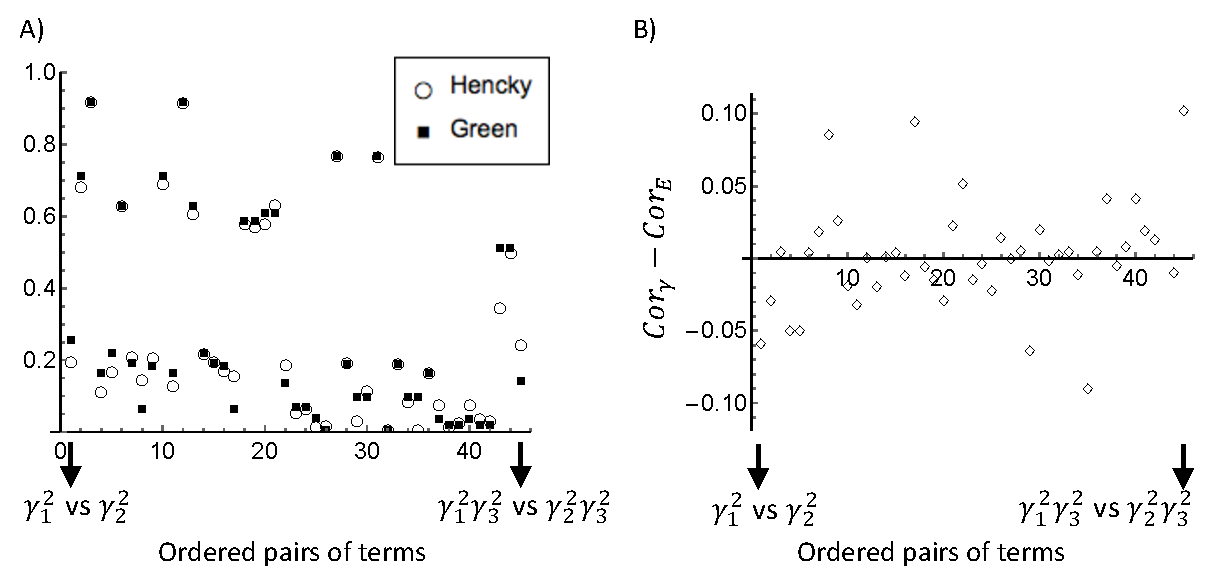
\includegraphics[width=6.0in]{Images/chapter5/gvsecorrelationeff}
\caption{(A) The correlation between parameters pairs in $\Psi_{eff}$ (Eqn. \ref{eqn:finalexponentialmodelformscaled}) when using Green-Lagrange vs Hencky strains. (B) The difference in correlation between each pair of parameters is minimal.}
\label{fig:gvsecorrelationeff}
\end{figure}
%-------------------	 end FIGURE 	-------------------%
%%%%%%%%%%%%%%%%%%%%%%%%%%%%%%%%%%%%%%%%%%%%%%%%%%%%%%%%%%%%


%%%%%%%%%%%%%%%%%%%%%%%%%%%%%%%%%%%%%%%%%%%%%%%%%%%%%%%%%%%%
%-------------------	begin FIGURE 	-------------------%
\begin{figure}
\centering
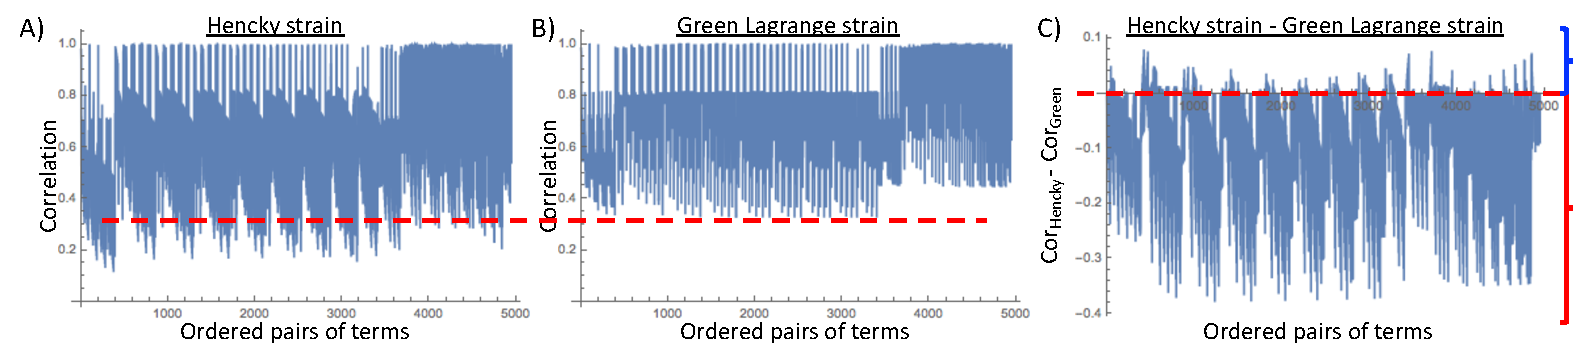
\includegraphics[width=\textwidth]{Images/chapter5/gvsecorrelationpoly}
\caption{(A) The correlation between parameters pairs in a polynomial series type model with powers up to 6 when using Green-Lagrange vs (B) Hencky strains. (C) The difference in correlation between each pair of parameters. The red bracketed terms are benefited from using Hencky strains whereas the significantly fewer blue bracketed terms has better correlations with Green-Lagrange strain.}
\label{fig:gvsecorrelationpoly}
\end{figure}
%-------------------	 end FIGURE 	-------------------%
%%%%%%%%%%%%%%%%%%%%%%%%%%%%%%%%%%%%%%%%%%%%%%%%%%%%%%%%%%%%
















%---    Discussion
\section{Optimal \textit{in silico} loading paths} \label{sec:optimalpaths}

	The most optimal loading path is the equibiaxial stress loading paths. This is not surprising as the equibiaxial stress response generally given very intuitive information on the mechanical response of soft tissues. Any odd number of loading paths will include the equibiaxial stress loading paths (Fig. \ref{fig:oddpaths}). Even when the number is even, we can observe that at least a few protocols are nearly equibiaxial in stress (Fig. \ref{fig:evenpaths}). For this reason, using an odd number of loading paths is highly recommended, as they will always include the minimal necessary set of loading paths, with the rest being average ratios in between (Fig. \ref{fig:oddpaths}). Even number of loading paths are generally very in consistent, and change slightly with each additional pairs of loading paths.  

%%%%%%%%%%%%%%%%%%%%%%%%%%%%%%%%%%%%%%%%%%%%%%%%%%%%%%%%%%%%
%-------------------	begin FIGURE 	-------------------%   
\begin{figure}
\centering
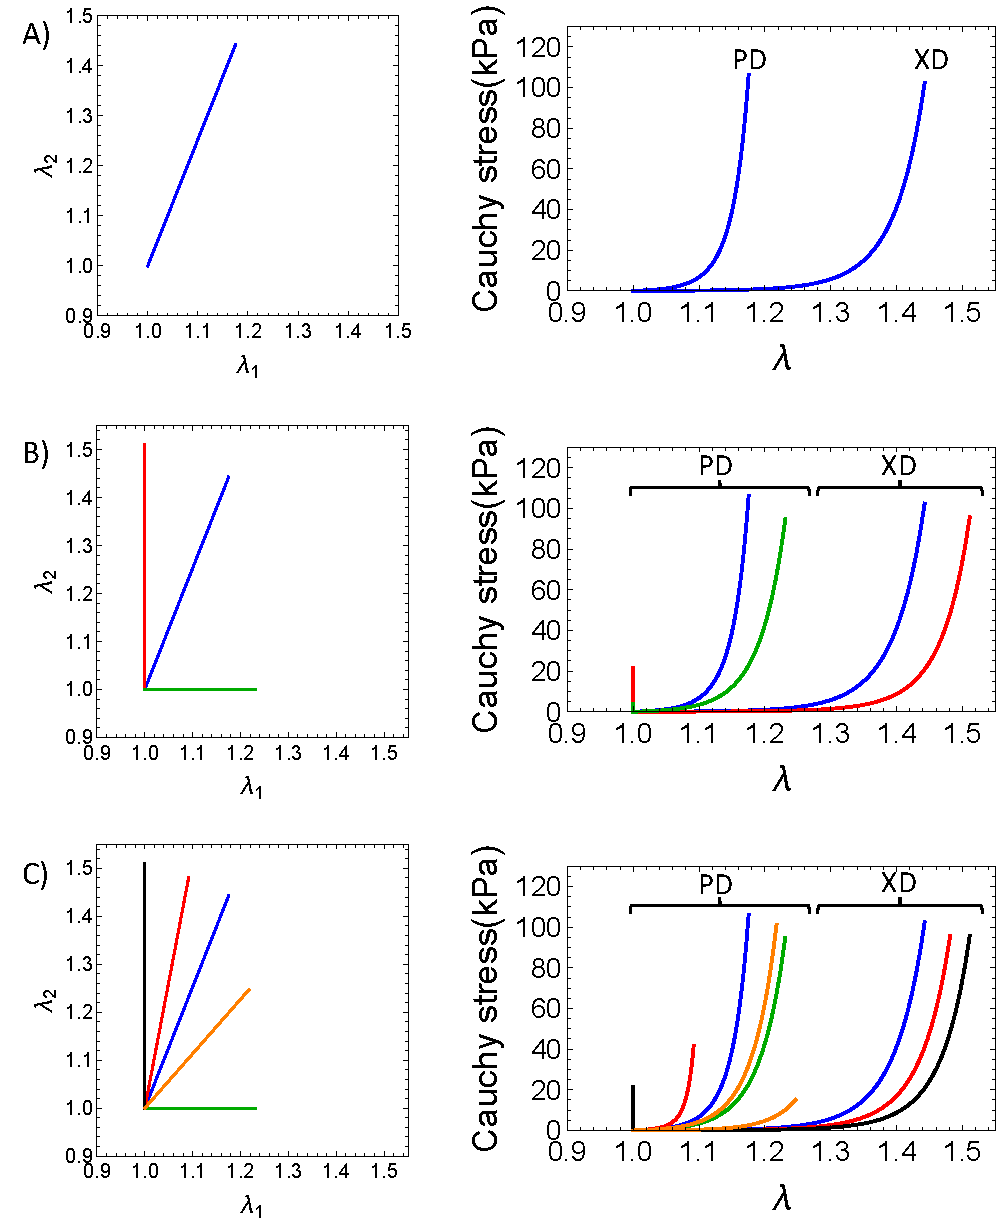
\includegraphics[width=5.5in]{Images/chapter5/oddpaths}
\caption{The optimal loading paths for generating data for a given total odd number of paths as well as the associated mechanical response, which is consistently containing the equi-biaxial stress loading path and the loading paths at the boundary.}
\label{fig:oddpaths}
\end{figure} 
%-------------------	 end FIGURE 	-------------------%
%%%%%%%%%%%%%%%%%%%%%%%%%%%%%%%%%%%%%%%%%%%%%%%%%%%%%%%%%%%%


%%%%%%%%%%%%%%%%%%%%%%%%%%%%%%%%%%%%%%%%%%%%%%%%%%%%%%%%%%%%
%-------------------	begin FIGURE 	-------------------%   
\begin{figure}
\centering
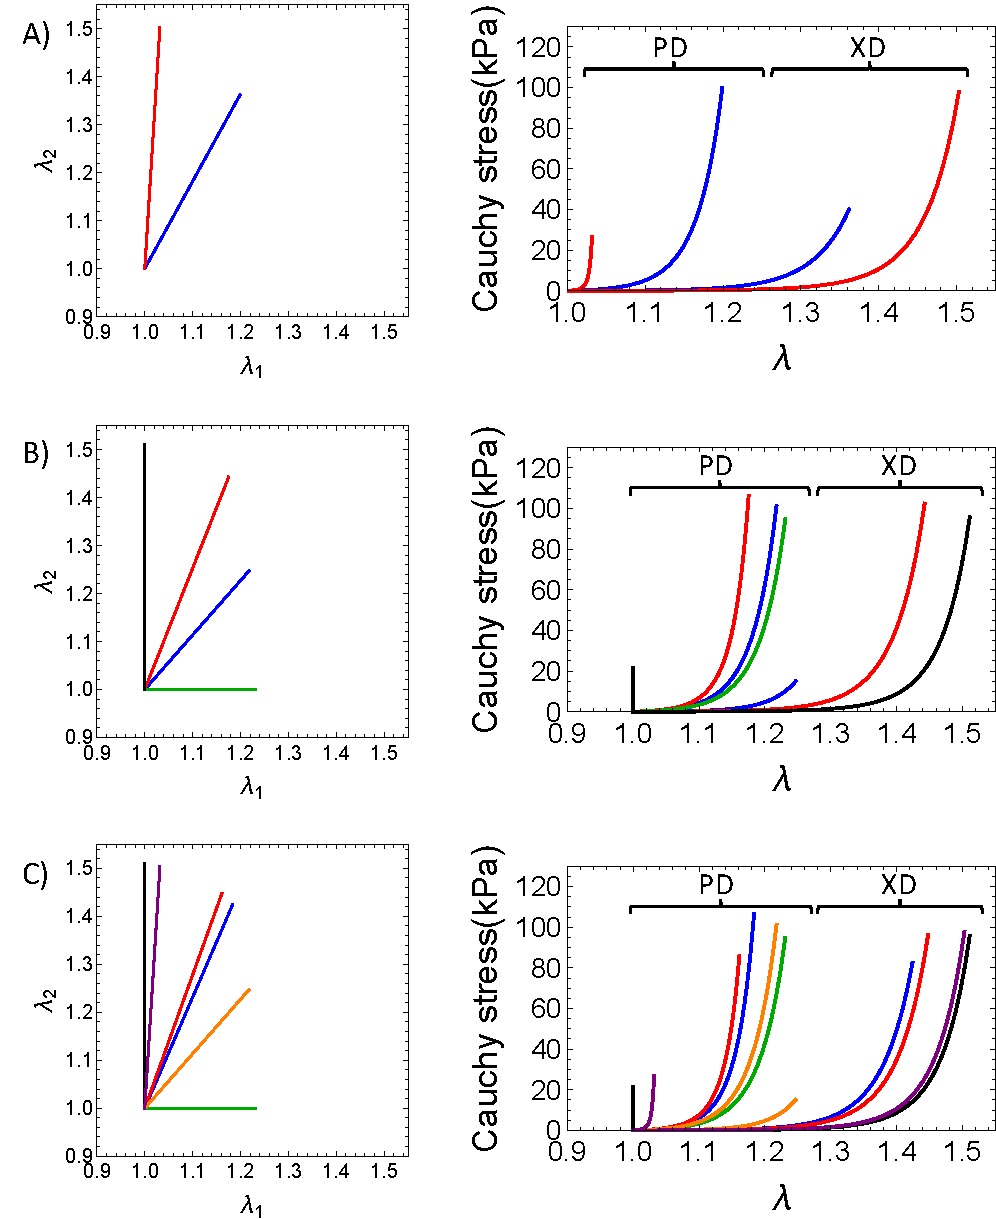
\includegraphics[width=5.5in]{Images/chapter5/evenpaths}
\caption{The optimal loading paths for generating data for a given even total number as well as the associated mechanical response, which is much more unpredictable than the odd (Fig. \ref{fig:oddpaths}) but gravitates towards the boundaries and the equi-biaxial loading paths as the number increases.}
\label{fig:evenpaths}
\end{figure} 
%-------------------	 end FIGURE 	-------------------%
%%%%%%%%%%%%%%%%%%%%%%%%%%%%%%%%%%%%%%%%%%%%%%%%%%%%%%%%%%%%

%---    Conclusion
\section{Additional results for other tissue types and effective constitutive model forms} \label{sec:otherresults}

	Bovine pericardium is a good soft tissue to start with due high axes stretch coupling from their broad fiber splays. However, soft tissue behavior is drastically different with greater degree and anisotropy. For example aortic valve leaflets have larger elastin content resulting in larger toe region and extremely narrow ODFs, which can cause contraction along the material axis under equi-biaxial tension \cite{billiar_biaxial_2000b}. This behavior is hard for most constitutive models to replicate. However, $\Psi_{eff}$ (Eqn. \ref{eqn:finalexponentialmodelformscaled}) has no problem replicating this behavior (Fig. \ref{fig:aorticfit}). 

%%%%%%%%%%%%%%%%%%%%%%%%%%%%%%%%%%%%%%%%%%%%%%%%%%%%%%%%%%%%
%-------------------	begin FIGURE 	-------------------%
\begin{figure}
\centering
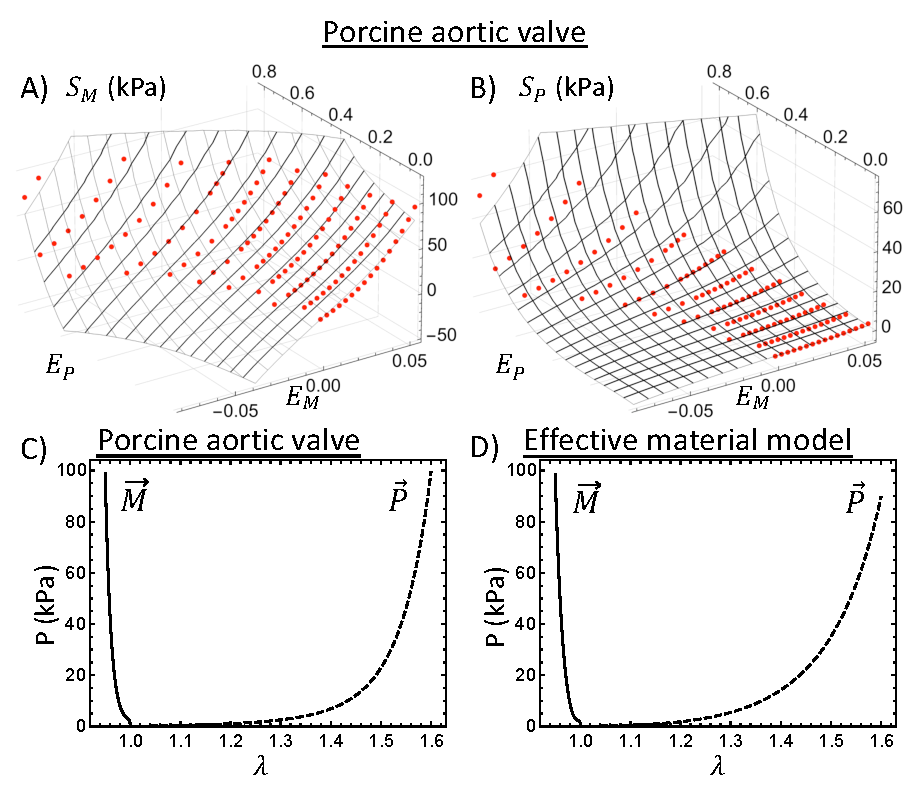
\includegraphics[width=\textwidth]{Images/chapter5/aorticfit}
\caption{Parameter estimation results for porcine aortic valve specimen with highly align collagen fibers, $\sigma_{ODF} =10\deg$. The response function A) $S_m$ and b) $S_n$ are shown. C) This specimen contracts in the preferred fiber direction under equi-biaxial tension, a trait of soft tissues with highly aligned collagen fibers. D) $\Psi_{eff}$ (Eqn. \ref{eqn:finalexponentialmodelformscaled}) is able to reproduce this effect.}
\label{fig:aorticfit}
\end{figure} 
%-------------------	 end FIGURE 	-------------------%
%%%%%%%%%%%%%%%%%%%%%%%%%%%%%%%%%%%%%%%%%%%%%%%%%%%%%%%%%%%%
    
    Based on D-optimality, we determined the optimal loading paths and shown its importance for model predictability. The equi-biaxial stress loading path (near equi-biaxial) came out as especially important, as it is included in all sets of optimal loading paths except for two and four (Fig. \ref{fig:oddpaths}\&\ref{fig:evenpaths}). Commonly, when reproducing results from older publication, only the equi-biaxial stress loading path may be included in the figures as it is the most informative. Indeed, using the equi-biaxial stress loading paths simply results in much higher D-optimality than other choices. However, using this loading path alone is not sufficient for parameter estimation. Although the quality of fit is very good (Fig. \ref{fig:effequifit}A\&B), it cannot predict other loading paths (Fig. \ref{fig:effequifit}C\&D) 
    
%%%%%%%%%%%%%%%%%%%%%%%%%%%%%%%%%%%%%%%%%%%%%%%%%%%%%%%%%%%%
%-------------------	begin FIGURE 	-------------------%
\begin{figure}[!hbtp]
\centering
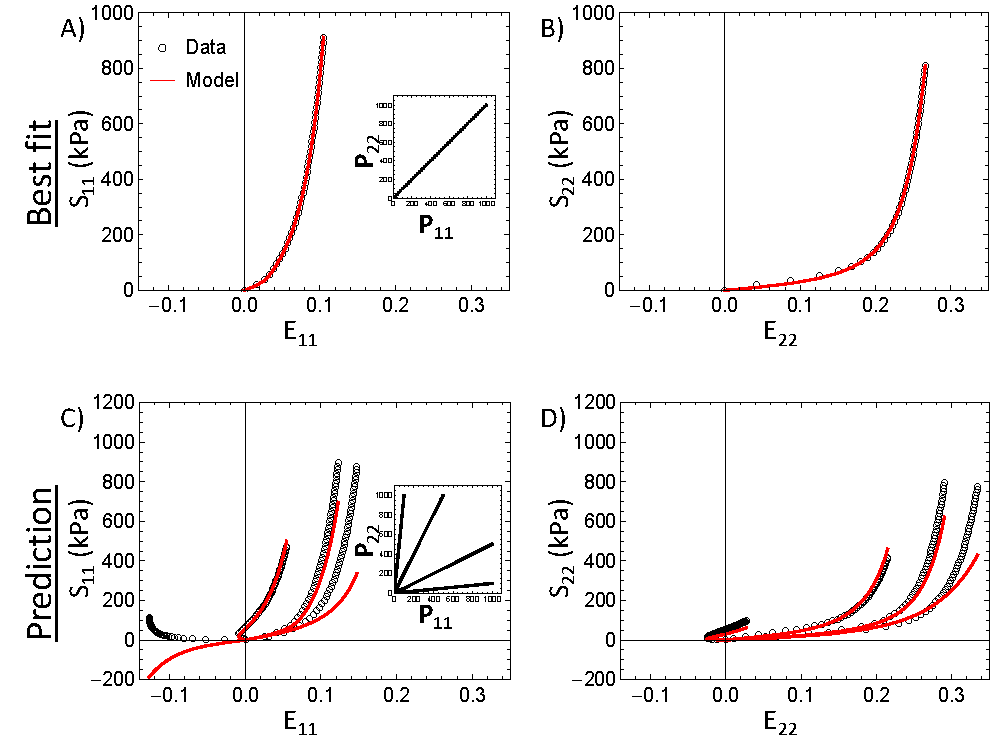
\includegraphics[width=\textwidth]{Images/chapter5/effequifit}
\caption{$\Psi_{eff}$ fitting to a single equi-biaxial loading path, showing the A) $S_{11}$ and B) $S_{22}$ component. The prediction for the C) $S_{11}$ component and D) $S_{22}$ component of the unfitted loading paths are poor. The inset in C shows the corresponding loading paths.}
\label{fig:effequifit}
\end{figure} 
%-------------------	 end FIGURE 	-------------------%
%%%%%%%%%%%%%%%%%%%%%%%%%%%%%%%%%%%%%%%%%%%%%%%%%%%%%%%%%%%%

	
%%%%%%%%%%%%%%%%%%%%%%%%%%%%%%%%%%%%%%%%%%%%%%%%%%%%%%%%%%%%
%-------------------	begin FIGURE 	-------------------%
\begin{figure}[!hbtp]
\centering
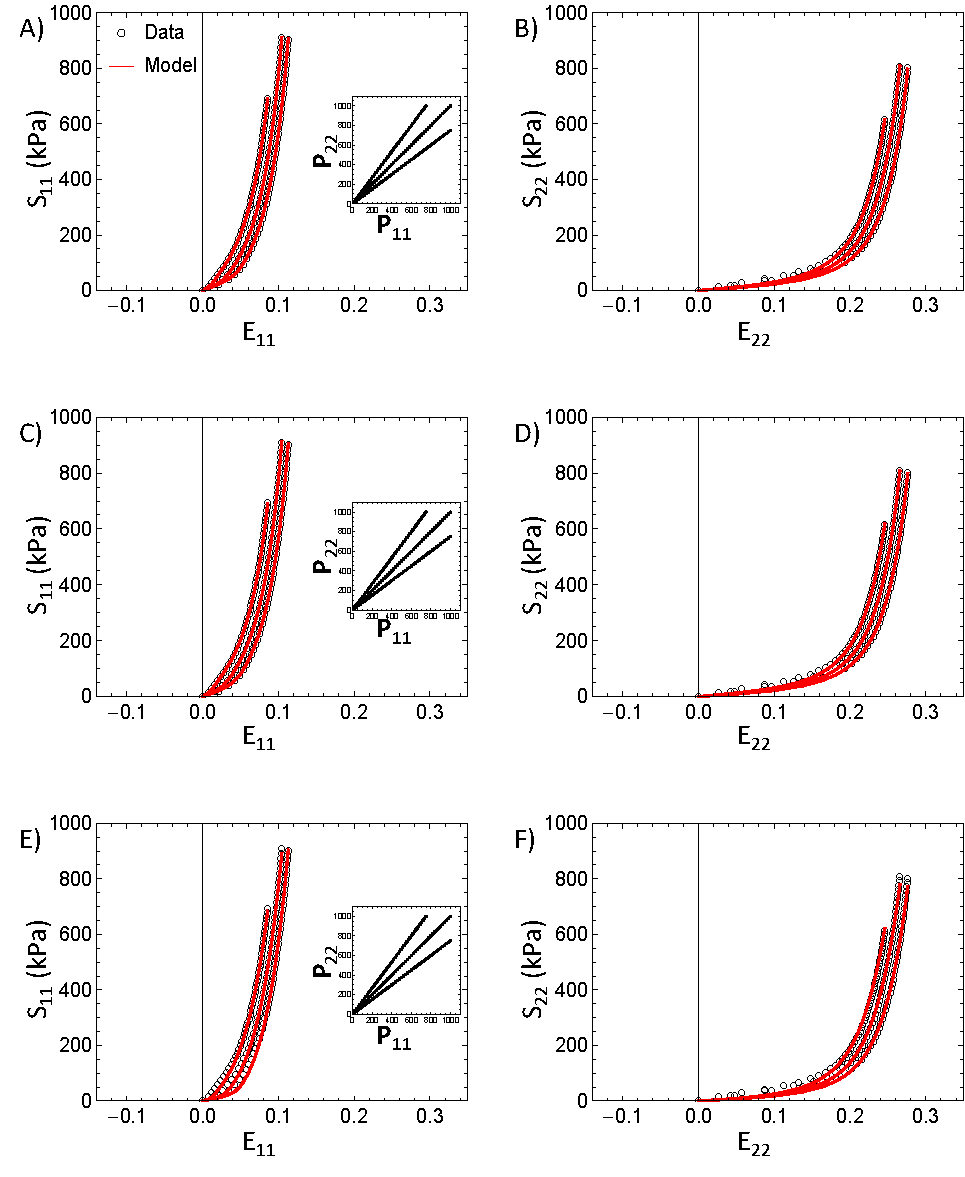
\includegraphics[width=\textwidth]{Images/chapter5/modelsfit}
\caption{All three models, A\&B) $\Psi_{eff}$ (Eqn. \ref{eqn:finalexponentialmodelformscaled}), C\&D) extended Fung (\ref{eqn:fullsunmodel}), and E\&F) the Sun model (\ref{eqn:extendedfung}), can fit the data equally as well.}
\label{fig:modelsfit}
\end{figure} 
%-------------------	 end FIGURE 	-------------------%
%%%%%%%%%%%%%%%%%%%%%%%%%%%%%%%%%%%%%%%%%%%%%%%%%%%%%%%%%%%%

%%%%%%%%%%%%%%%%%%%%%%%%%%%%%%%%%%%%%%%%%%%%%%%%%%%%%%%%%%%%
%-------------------	begin FIGURE 	-------------------%
\begin{figure}[!hbtp]
\centering
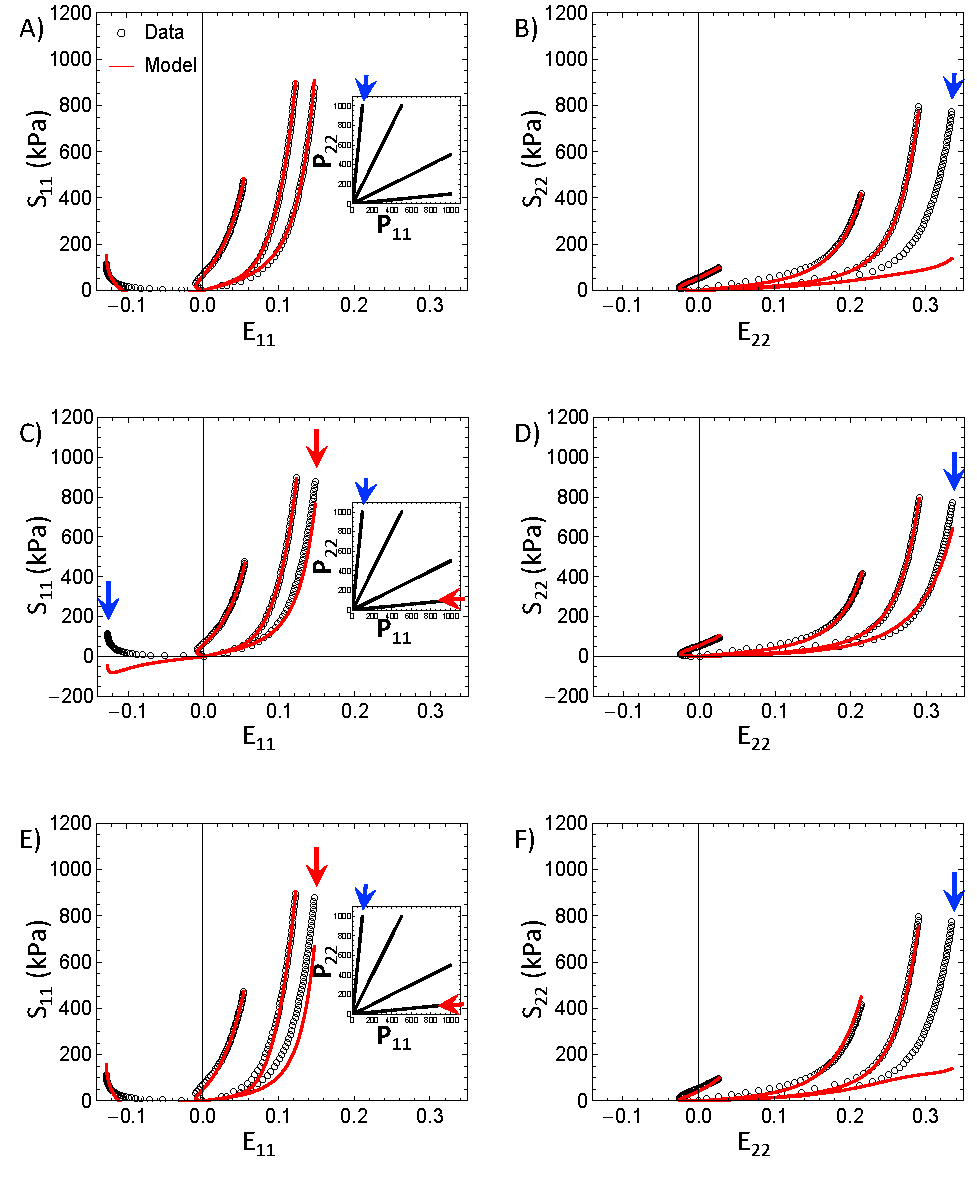
\includegraphics[width=\textwidth]{Images/chapter5/modelspred}
\caption{The predictions for the unfitted loading paths from Fig. \ref{fig:modelsfit}. The blue and red arrows points out the poorly predicted paths, and which path they are on the inset figures.}
\label{fig:modelspred}
\end{figure} 
%-------------------	 end FIGURE 	-------------------%
%%%%%%%%%%%%%%%%%%%%%%%%%%%%%%%%%%%%%%%%%%%%%%%%%%%%%%%%%%%%


    With the addition of other loading paths, even non-optimal, this can significantly improve the predictive capabilities (Fig. \ref{fig:modelspred}A\&B). However, we can clearly see that because the loading paths are not optimal, the $0.1/1$ loading path is not predicted very well (Fig. \ref{fig:modelspred}B). We tested to see if this can be improved through more specific forms of $\Psi_{eff}$ (Eqn. \ref{eqn:finalexponentialmodelformscaled}). For this, we looked at an extension of the generalized Fung model to quadratic terms presented by Sun \textit{et al.} \cite{sun_biaxial_2003} to better fit the response of the glutaraldehyde cross-linked bovine pericardium. The additional terms are only of cubic and quartic powers, $B_{ijkl}E_{ij}^2E_{kl}^2$. In comparison to $\Psi_{eff}$, this is only missing $E_m^3E_n$ and $E_m^3E_n$,
%==========================================================%
%-------------------	begin EQUATION 	-------------------%
\begin{equation}\label{eqn:fullsunmodel}
\begin{aligned}
\Psi	=& c_0 \left(e^{Q} - 1\right) \\
Q		=& A_1 E_{11}^2 + A_2 E_{22}^2 + 2A_3E_{11}E_{22} + A_4 E_{12}^2 + 2A_5E_{12}E_{11}	\\
	&+ 2A_6E_{12}E_{22} + B_1 E_{11}^4 + B_2 E_{22}^4 + 2B_3E_{11}^2E_{22}^2 + B_4 E_{12}^4	\\
    &+ 2B_5E_{12}^2E_{11}^2 + 2B_6E_{12}^2E_{22}^2 
\end{aligned}\tag{Sun et al. \cite{sun_biaxial_2003} Eqn. 4}
\end{equation}
%-------------------	 end EQUATION 	-------------------%
%==========================================================%   
We will call this the extended Fung model. In addition, Sun \textit{et al.} \cite{sun_biaxial_2003} also recommended a more minimalistic form, where only the coupling term $2B_3E_{11}^2E_{22}^2$ is added as , 
%==========================================================%
%-------------------	begin EQUATION 	-------------------%
\begin{equation}\label{eqn:extendedfung}
\begin{aligned}
\Psi	=& c_0 \left(e^{Q} - 1\right) \\
Q		=& A_1 E_{11}^2 + A_2 E_{22}^2 + 2A_3E_{11}E_{22} + A_4 E_{12}^2 + 2A_5E_{12}E_{11}	\\
	&+ 2A_6E_{12}E_{22} + 2B_3E_{11}^2E_{22}^2 + B_4 E_{12}^4.
\end{aligned}
\end{equation}
%-------------------	 end EQUATION 	-------------------%
%==========================================================% 
    We shall call this the Sun model. 

	Although the equality of fit are all equally as good \ref{fig:modelsfit}, the extended Fung model (Eqn. \ref{eqn:fullsunmodel}) predicts $S_{22}$ component of the 0.1/1 loading path much better, but predicts the wrong sign for $S_{11}$ for the same loading path, as well as predicting the 1/0.1 loading path worse (Fig. \ref{fig:modelspred}C\&D). The Sun model (Eqn. \ref{eqn:extendedfung}) on the other hand is similar to $\Psi_{eff}$ but worse at predicting $S_{11}$ of the 1/0.1 loading path (Fig. \ref{fig:modelspred}E\&F). It's hard to predict how these constitutive models will behave when the loading paths are not optimal. This is especially true when only a single protocol is used, where predictions for all other protocols can be very poor (Fig. \ref{fig:effequifit}). However, as little as three loading paths are needed to fully reproduce the mechanical response of soft tissue over the entire range of deformations (Fig. \ref{fig:effoptpred}).





%---    Bioliography
\bibliographystyle{plainnat}
\bibliography{phd}